\documentclass[a4paper,11pt]{article}
%
%--------------------   start of the 'preamble'
%
\usepackage{graphicx,amssymb,amstext,amsmath}
%
%%    homebrew commands -- to save typing
\newcommand\etc{\textsl{etc}}
\newcommand\eg{\textsl{eg.}\ }
\newcommand\etal{\textsl{et al.}}
\newcommand\Quote[1]{\lq\textsl{#1}\rq}
\newcommand\fr[2]{{\textstyle\frac{#1}{#2}}}
\newcommand\miktex{\textsl{MikTeX}}
\newcommand\comp{\textsl{The Companion}}
\newcommand\nss{\textsl{Not so Short}}
%
%---------------------   end of the 'preamble'
%
\begin{document}
%-----------------------------------------------------------
\title{Report of MSR Data Mining Challenge 2012}
\author{Laura Bledaite \& Martynas Pumputis}
\maketitle
%-----------------------------------------------------------
%\tableofcontents
%-----------------------------------------------------------
\section{Introduction}
In this report we describe the outcomes of analysis when working with the data provided by the MSR 2012 Data Mining Challenge. The data contains the change and bug report data for the Android platform. In the second section of the report we report some statistics about the data and in the third one we introduce our own buggy files' detection analysis approch.

\section{Simple Statistics}
First of all, we tried to make some statistics about the data in order to see how it looks and get some ideas about what might be done and/or draw some conclusions.
The first thing we looked at was the comment frequencies in a bug. We have 14975 comments related to some bug in total. The maximum number of comments related to one bug was 25, the minimum - 1, the average - 4.5228714524207. The graph showing the distribution of the comment frequencies in a bug is shown in Figure~\ref{fig:com_freq}. This lets us conclude that most of the bugs do not have many comments, most often they have only one or a couple of them. Actually, 79\% of the bugs have $<=5$ comments.

\begin{figure}[ht!]
\centering
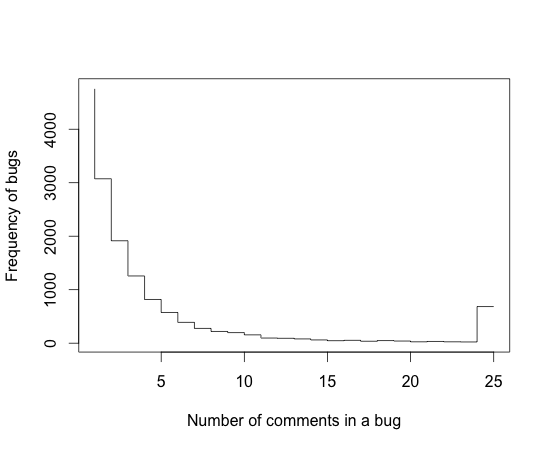
\includegraphics[width=.7\textwidth]{../diagrams/comment_frequencies.png}
\caption{Comment frequencies in a bug.}
\label{fig:com_freq}
\end{figure}

Secondly, we were interested in how long it takes to solve a bug. In order to find it, we filtered the data taking only the bugs that are already closed and calculates the times from opening untill closing in days. There were 6345 closed bugs. The minimum time required to solve the bug took 0.0001967591 days, maximum - 1365.347, average - 72.44017. Figure~\ref{fig:res_times} shows the distribution of the time required for resolving a bug.

\begin{figure}[ht!]
\centering
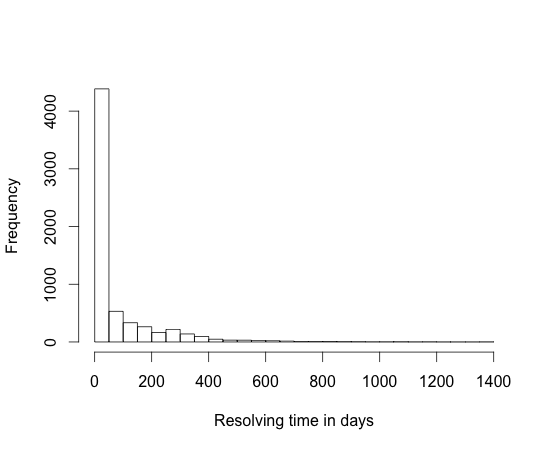
\includegraphics[width=.7\textwidth]{../diagrams/resolving_times.png}
\caption{Histogram of bug resolving times.}
\label{fig:res_times}
\end{figure}
 
Moving more in detail, we made an assumption that maybe the resolving time and the number of comments are related, i.e. maybe there exists a tendency that more comments mean faster resolving of a bug. Figure~\ref{fig:com_time} shows the relationship between the number of comments in a bug and the time required to resolve a bug. A line in Figure~\ref{fig:com_time} shows an attempt to adjust the linear regression model for the data using the number of comments as a predictor variable.

\begin{figure}[ht!]
\centering
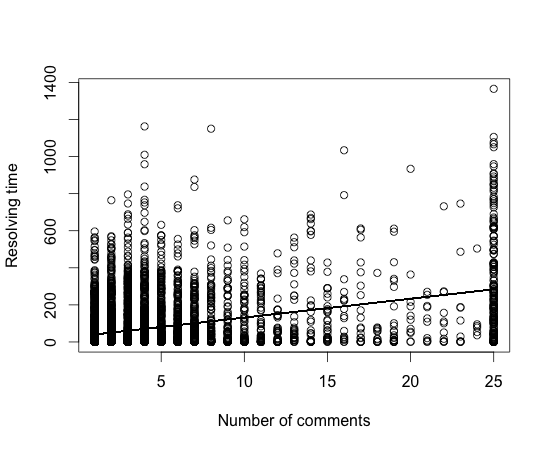
\includegraphics[width=.7\textwidth]{../diagrams/comments_time.png}
\caption{Bug resolving time realtionship with the number of comments in a bug.}
\label{fig:com_time}
\end{figure}

The predicted model looks like this:
\[
ResolvingTime=30.0465 + 10.1493 \cdot NumberOfComments.\]
The results of the general linear model are shown in Table~\ref{tbl:glm}.

\begin{table}[ht!]
\centering
\begin{tabular}{|c|c|c|c|c|c|c|}
\hline
Coefficients & Estimate Std. & Error & t value & {$Pr(>|t|)$}\tabularnewline
\hline
\hline
(Intercept) & 30.0465 & 2.0509 & 14.65 & {$<2e-16 $}***\tabularnewline
\hline
NumberOfComments & 10.1493 & 0.3108 & 32.66 & {$<2e-16$}***\tabularnewline
\hline
\end{tabular}
\footnotemark{Signif. codes:  *** 0.001 ** 0.01 * 0.05}
\caption{Linear regression results.}
\label{tbl:glm}
\end{table}

Inspite of the fact, that the results of the general linear model prove the coefficient of the number of comments not be be equal 0, the data do not seem to be very well explained by the model adjusted. This might have happened because it may happen naturally, that the longer the bug is being solved, the more comments it gets, but it does not give any more information. Contrarily, we expect that the more comments a bug gets, the faster it is resolved. To address this issue, we decided to take a look at the comments' density in a time period and its relationship to the resolving time. 

\begin{figure}[ht!]
\centering
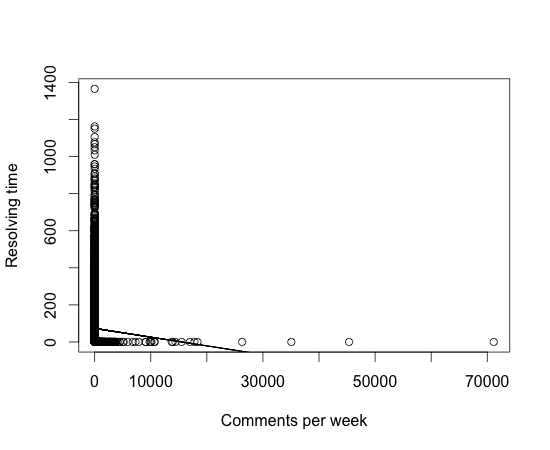
\includegraphics[width=.7\textwidth]{../diagrams/density_time.png}
\caption{Bug resolving time realtionship with the comment density in a bug.}
\label{fig:density_time}
\end{figure}

And actually results show that there exist such a relationship. Figure~\ref{fig:density_time} does not suggest the fitting model for the data, but it shows several data properties. Firstly, it is easy to notice that whenever a bug is very dense in comments, it will most likely be resolved very fast. On the other hand, it does not mean that a bug which is sparse in comments cannot be resolved fast. Bugs having few comments have similar probability to be solved fast or slow.

One more thing we analysed, was the origin of the programmers. We divided them according to the timezones they were working in and got quite interesting results. Figure~\ref{fig:time_zones} shows the distribution of the time zones the Android programmers were working in. From the results we can see that the programmers from the West coast of the USA(time zones -8 and -7) are most active. The second most active cluster of coders are from Europe(time zones 0, 1 and 2). The third most active group comes from the East side of USA and/or South America plus Greenland :) (time zones -5, -4 and -3). And the last group of active programmers is located in East Asia and/or Australia (time zones 8, 9 and 10). The relation between the programmers activity and the time zones can be seen from Figure~\ref{fig:time_zones} and Figure~\ref{fig:tz_map}

\begin{figure}[ht!]
\centering
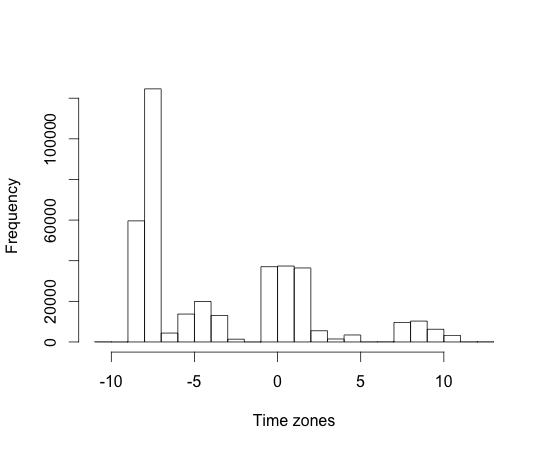
\includegraphics[width=.7\textwidth]{../diagrams/time_zones.png}
\caption{Histogram of the time zones of the coders.}
\label{fig:time_zones}
\end{figure}

\begin{figure}[ht!]
\centering
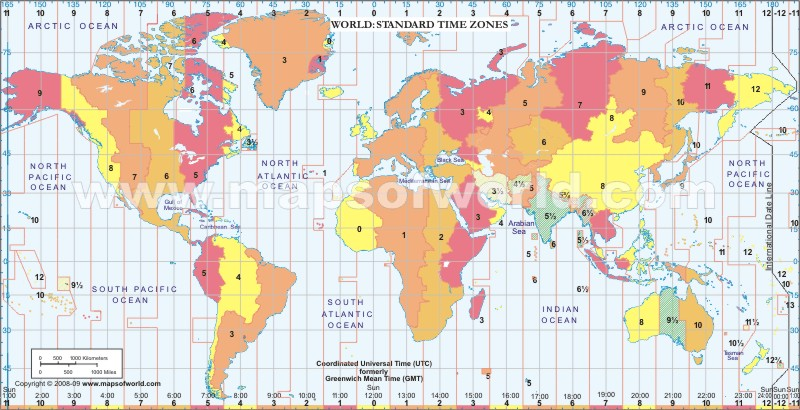
\includegraphics[width=1.2\textwidth]{../diagrams/World-Time-Zone.jpg}
\caption{World Time Zones~\cite{map}.}
\label{fig:tz_map}
\end{figure}

\section{Buggy Files' Analysis}

There are 387527 commits in a dataset git.log.xml, 381736 of them have authors. There are 11310 distinct authors. Each commit in git.log.xml contains a message which could link to some bug
(i.e. bug id). We used /Bug.*?(\d+)/ regular expression pattern to recognize such messages. Also
each message lists files that were changed in commit.

We can make an
assumption - if commit has a bug id then all files changed in commit fixes the
bug, so these files before the commit was made contained the bug.

Listed files are in form of absolute paths. For each ancestor directory of a file
we applied some weight. Formula for calculating a weight:
\[Weight = \frac{\#PathParts^2}{SumOfAllParts^2}\] E.g.
'/foo/bar/yadda' can be divided into '/foo/bar/yadda', '/foo/bar' and '/foo'
subpaths and '/foo/bar/yadda' weight is equal to {$\frac{3^2}{(3+2+1)^2} = \frac{1}{4}$}

After appyling Map-Reduce algorithm for calculating path weights, we got a
histogram depicted in Figure~\ref{fig:bug_files}

\begin{figure}[ht!]
\centering
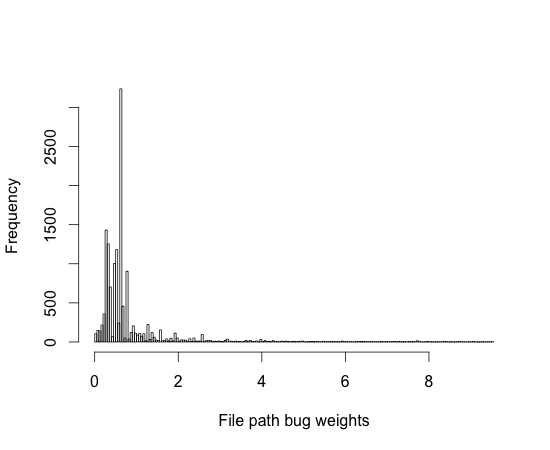
\includegraphics[width=1.2\textwidth]{../diagrams/bug_files.png}
\caption{Weights of file paths.}
\label{fig:bug_files}
\end{figure}

Then we calculated a 95 \%quantile and using it decided to consider a path buggy if its weight exceeds this value. 

\[95\%quantile(PathWeights) = 2.509803922\]

Assuming this we concluded that there exist 1459 commits (out of 3600 with the set bug id) that are probably buggy.

Table~\ref{tbl:weights} lists the heaviest files (highest probability that they contained bugs).

\begin{table}[ht!]
\centering
\begin{tabular}{|c|c|}
\hline
File & Weight\tabularnewline
\hline
\hline
src/com/android/contacts/TwelveKeyDialer.java & 9.54545454545454\tabularnewline
\hline
libcore/luni/src/test/java & 9.49488061963582\tabularnewline
\hline
tests/src/com/android/providers & 9.46428571428572\tabularnewline
\hline
src/com/android/tradefed & 9.43296703296703\tabularnewline
\hline
src/main/java/com/google/gerrit/client/admin & 9.43157894736842\tabularnewline
\hline
tests/tests/app/src/android/app/cts & 9.36764705882353\tabularnewline
\hline
tools/host/src/com/android & 9.28571428571429\tabularnewline
\hline
\end{tabular}
\caption{Heaviest files with their weights.}
\label{tbl:weights}
\end{table}

We used the previous results for identifying commits that could introduce a
bug. We calculated commit weight (i.e. sum  of the weights of its files from bug
list). Figure~\ref{fig:commit_weights} shows the histogram of the commit weights.

\begin{figure}[ht!]
\centering
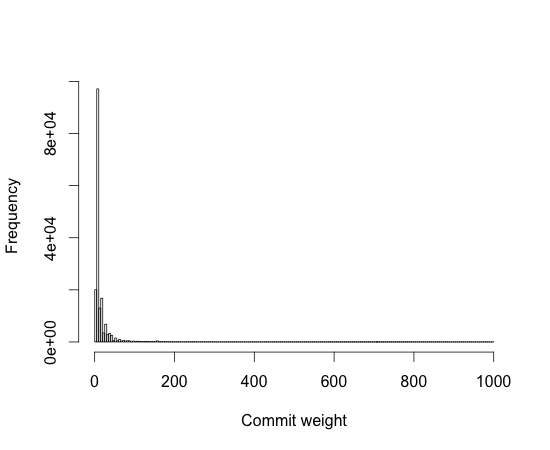
\includegraphics[width=1.2\textwidth]{../diagrams/commit_weight.png}
\caption{Weights of the commits.}
\label{fig:commit_weights}
\end{figure}

Again we calculated a 95 \%quantile of the commit weights
\[95\%quantile(CommitWeights) = 51.10859\] and found that 8870 commits (out of 383296 with a set bug id) exceed the quantile and  hence might be buggy.

Using this data, it is possible to find the authors, that might have introduced the bugs (assuming their commits had the highest weights). Table~\ref{tbl:bad_authors} lists the authors of the commits with the highest commit weight.

\begin{table}[ht!]
\centering
\begin{tabular}{|c|c|}
\hline
Author & Commit Weight\tabularnewline
\hline
\hline
enf@google.com & 71201.9323689457\tabularnewline
\hline
bzolnier@gmail.com & 67698.4585414578\tabularnewline
\hline
initial-contribution@android.com & 65777.331943003\tabularnewline
\hline
gregkh@suse.de & 60382.0305083022\tabularnewline
\hline
 & 45167.6397066183\tabularnewline
\hline
sop@google.com & 29901.0723573367\tabularnewline
\hline
htejun@gmail.com & 25401.5209457247\tabularnewline
\hline
khali@linux-fr.org & 24971.6075258094\tabularnewline
\hline
tiwai@suse.de & 24227.9363969302\tabularnewline
\hline
joe@perches.com & 21284.0999999987\tabularnewline
\hline
\end{tabular}
\caption{Authors of the commits with the highest weight.}
\label{tbl:bad_authors}
\end{table}

Table~\ref{tbl:fast_authors} lists the most frequent commiters, i.e. the commit authors that make the commits most frequently, and their commit weights. Table~\ref{tbl:bad_authors} and Table~\ref{tbl:fast_authors} enables the comparison between the 'likely-to-be-buggy' commit authors and the most frequent commit authors.

\begin{table}[ht!]
\centering
\begin{tabular}{|c|c|}
\hline
Author & Commit Weight\tabularnewline
\hline
\hline
android-gerrit@google.com & 10377\tabularnewline
\hline
torvalds@linux-foundation.org & 6857\tabularnewline
\hline
 & 5791\tabularnewline
\hline
initial-contribution@android.com & 4262\tabularnewline
\hline
jbq@google.com & 4044\tabularnewline
\hline
marcel@holtmann.org & 3773\tabularnewline
\hline
xav@android.com & 3492\tabularnewline
\hline
mingo@elte.hu & 3390\tabularnewline
\hline
sop@google.com & 3274\tabularnewline
\hline
tiwai@suse.de & 3062\tabularnewline
\hline
\hline
\end{tabular}
\caption{Most frequent commiters.}
\label{tbl:fast_authors}
\end{table}

Note that some of the commits did not have their author. Hence the is a line with non existing author in both Table~\ref{tbl:bad_authors} and Table~\ref{tbl:fast_authors}. The autors that fall into both categories include initial-contribution@android.com, sop@google.com and tiwai@suse.de. It means that not necessarily the ones that commit most frequently, also make bugs most frequently and therefore might differentiate the fast and reliable commiters from the not so fast and not so reliable ones.

%-----------------------------------------------------------
\addcontentsline{toc}{chapter}{\numberline{}Bibliography}

\begin{thebibliography}{9999}%\enlargethispage{\baselineskip}
\bibitem{map} http://www.mapsofworld.com
\end{thebibliography}
\vfill
\begin{flushright}\small Prepared in \LaTeXe\ \end{flushright}

%-----------------------------------------------------------
\appendix
\section{Entity-Relationship Diagram of Android Commits and Bugs.}
\begin{figure}[ht!]
\centering
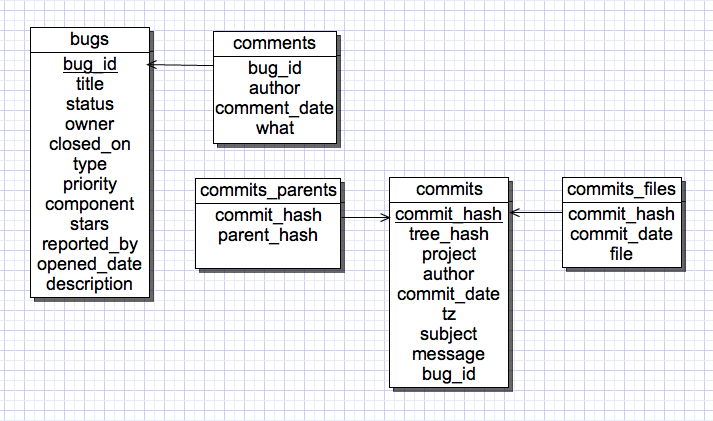
\includegraphics[width=1.2\textwidth]{../diagrams/er_diagram.png}
%\caption{Android commits and bugs.}
\label{fig:er_diagram}
\end{figure}

%-----------------------------------------------------------
\end{document}
